\documentclass[10pt]{article}
\usepackage[utf8]{inputenc}
\usepackage[activeacute,spanish]{babel}
\usepackage[left=1.5cm,top=1.5cm,right=1.5cm, bottom=1.5cm,letterpaper, includeheadfoot]{geometry}

\usepackage{amssymb, amsmath, amsthm}
\usepackage{graphicx}
\usepackage{hyperref}
\usepackage{lmodern,url}
\usepackage{paralist} %util para listas compactas
\usepackage{xcolor}
\usepackage{bbm}
\usepackage{mathrsfs}
\usepackage{bbm}

%========PAQUETES AGREGADOS===========
%Pseudocodigo
\usepackage{pseudocode}
\usepackage[portuguese, boxruled]{algorithm2e}
\usepackage{wrapfig}
\usepackage{multicol}
\usepackage{graphicx}
\usepackage{caption}
\usepackage{subcaption}
%\captionsetup[table]{labelformat=empty}
\captionsetup[subfigure]{labelformat=empty}
\usepackage{cancel}
\usepackage{tikz}
\def\checkmark{\tikz\fill[scale=0.4](0,.35) -- (.25,0) -- (1,.7) -- (.25,.15) -- cycle;} 
%====================================

\usepackage{fancyhdr}
\pagestyle{fancy}
\fancypagestyle{plain}{%
\fancyhf{}
\lhead{\footnotesize\itshape\bfseries\rightmark}
\rhead{\footnotesize\itshape\bfseries\leftmark}
}


% macros
\newcommand{\Q}{\mathbb Q}
\newcommand{\R}{\mathbb R}
\newcommand{\N}{\mathbb N}
\newcommand{\Z}{\mathbb Z}
\newcommand{\C}{\mathbb C}
\newcommand{\BigO}{\mathcal{O}}
%Teoremas, Lemas, etc.
\theoremstyle{plain}
\newtheorem{teo}{Teorema}
\newtheorem{lem}{Lema}
\newtheorem{prop}{Proposición}
\newtheorem{cor}{Corolario}
\newtheorem{obs}{Observación}
\newtheorem{ej}{Ejemplo}
\renewcommand{\qedsymbol}{\rule{0.7em}{0.7em}}
\renewenvironment{proof}{{\bfseries \noindent Demostración}}{ \qed \\}


\theoremstyle{definition}
\newtheorem{defi}{Definición}
% fin macros


\newcommand{\catnum}{13} %numero de catedra
\newcommand{\fecha}{13 de Septiembre 2016 }

%%%%%%%%%%%%%%%%%%

%Macros para este documento
\newcommand{\cin}{\operatorname{cint}}



\begin{document}
%Encabezado
\fancyhead[L]{Facultad de Ciencias Físicas y Matemáticas}
\fancyhead[R]{Universidad de Chile}
\vspace*{-1.2 cm}
\begin{minipage}{0.6\textwidth}
\begin{flushleft}
\hspace*{-0.5cm}\textbf{MA3402-1 Estadística. Primavera 2016}\\
\hspace*{-0.5cm}\textbf{Profesor:} Raul Gouet\\
\hspace*{-0.5cm}\textbf{Escriba:} Manuel Cáceres\\
\hspace*{-0.5cm}\textbf{Fecha:} \fecha
\end{flushleft}
\end{minipage}
\begin{minipage}{0.36\textwidth}
\begin{flushright}

\includegraphics[scale=0.3]{imagenes/fcfm_dcc}
\end{flushright}
\end{minipage}
\bigskip
%Fin encabezado

\begin{center}
\LARGE\textbf{Clase \catnum}
\end{center}
\section{Comparación de poblaciones normales}
Se trata de comparar 2 distribuciones normales, digamos $N(\mu,\sigma^2), N(\nu,\tau^2)$. Tenemos $X_{1},\ldots,X_{m}$ iid $N(\mu,\sigma^2)$, $Y_{1},\ldots,Y_{n}$ iid $N(\nu,\tau^2)$. y queremos saber $H_{0}: \mu = \nu, \sigma = \tau$ versus $H_{1}: No!$.\\

Una de las más importantes corresponde a la comparación de medias (o valores esperados).\\

El problema se plantea como: $H_{0}: \mu=\nu$ versus $H_{1}:\mu \not = \nu$.\\
Este problema que no menciona las varianzas al plantearlo con $\sigma,\tau$ conocidos es sencillo.\\
Pero si $\sigma,\tau$ son desconocidos entonces hay dificultades técnicas.\\

Se puede comenzar suponiendo $\sigma =\tau$.\\

El problema que estudiaremos es $H_{0}: \mu=\nu$ versus $H_{1}:\mu \not = \nu$ con $\sigma=\tau$ desconocido.\\

Tenemos $X_{1},\ldots,X_{m}$ iid $N(\mu,\sigma^2)$, $Y_{1},\ldots,Y_{n}$ iid $N(\nu,\tau^2)$.\\

\begin{align*}
\lambda(X,Y) &= \frac{\sup_{\theta \in \Theta}f_{\theta}(X,Y)}{\sup_{\theta \in \Theta_{0}}f_{\theta}(X,Y)}\\
\Theta &= \{(\mu,\nu,\sigma)\colon \mu,\nu \in \mathbb{R}, \sigma>0\}\\
\Theta_{0} &= \{(\mu,\mu,\sigma)\colon \mu \in \mathbb{R}, \sigma>0\}
\end{align*} 
Calculamos los supremos, para lo cual buscamos los EMV de los parámetros:
\begin{align*}
(X,Y) =& (X_{1},\ldots,X_{m},Y_{1},\ldots,Y_{n}) =: Z\\
f_{\theta}(X,Y) &= \left(\frac{1}{\sqrt{2\pi}\sigma}\right)^me^{-\frac{1}{2\sigma^2}\sum (X_{i}-\mu)^2} \left(\frac{1}{\sqrt{2\pi}\sigma}\right)^ne^{-\frac{1}{2\sigma^2}\sum (Y_{i}-\nu)^2}
\end{align*}
Calculemos $\sup_{\mu,\nu,\sigma}f_{\theta}(X,Y)$
\begin{align*}
\log f_{\theta} &= k - \frac{1}{2\sigma^2}\sum (X_{i}-\mu)^2 - \frac{1}{2\sigma^2}\sum (Y_{i}-\nu)^2\\
\frac{\partial \log f_{\theta}}{\partial \mu} &= c\sum(X_{i}-\mu) = 0 \Rightarrow \hat{\mu} = \bar{X}\\
\frac{\partial \log f_{\theta}}{\partial \nu} &= c\sum(Y_{i}-\nu) = 0 \Rightarrow \hat{\nu} = \bar{Y}\\
\frac{\partial \log f_{\hat{\mu},\hat{\nu},\sigma}}{\partial \sigma} &= \frac{-n+m}{\sigma} + \frac{1}{\sigma^3}\sum (X_{i}-\bar{X})^2 + \frac{1}{\sigma^3}\sum (Y_{i}-\bar{Y})^2 = 0\\
\Rightarrow & \hat{\sigma}^2 = \frac{1}{n+m}\left(\underbrace{\sum (X_{i}-\bar{X})^2}_{m\hat{\sigma_{X}}} + \underbrace{\sum (Y_{i}-\bar{Y})^2}_{n\hat{\sigma_{Y}}}\right)\\
&= \frac{m\hat{\sigma_{X}}+n\hat{\sigma_{Y}}}{n+m} \text{ promedio ponderado de las varianzas}\\
f_{\hat{\mu},\hat{\nu},\hat{\sigma}}(X,Y) &= k\hat{\sigma}^{-(n+m)}e^{-\frac{m+n}{2}}
\end{align*}
que corresponde al numerador de $\lambda$.\\

Estudiemos ahora $\sup_{\mu,\sigma}f_{\mu,\mu,\sigma}(X,Y)$.
\begin{align*}
\log f_{\mu,\mu,\sigma} &= k- (m+n)\log \sigma - \frac{1}{2\sigma^2}\left(\sum (X_{i}-\mu)^2+\sum (Y_{i}-\mu)^2\right)\\
\frac{\partial \log}{\partial \mu} &= c\left(\sum (X_{i}-\mu + \sum (Y_{i}-\nu))\right) = 0\\
\Rightarrow &\tilde{\mu} = \frac{1}{m+n}\left(\sum X_{i}+ \sum Y_{i}\right) = \frac{m\bar{X}+n\bar{Y}}{m+n} \text{ promedio ponderado de las medias}\\
\frac{\partial \log f_{\tilde{\mu},\tilde{\mu},\sigma}}{\partial \sigma} &= -\frac{m+n}{\sigma} + \frac{1}{\sigma^2}\left(\sum (X_{i}-\hat{\mu})^2+\sum (Y_{i}-\hat{\mu})^2\right)  = 0\\
\Rightarrow & \hat{\sigma}^2 = \frac{1}{m+n}\left(\sum (X_{i}-\hat{\mu})^2+\sum (Y_{i}-\hat{\mu})^2\right)\\
f_{\tilde{\mu},\tilde{\mu},\sigma} &= k \tilde{\sigma}^{-(m+n)}e^{-\frac{m+n}{2}}
\end{align*}
que corresponde al denominador de $\lambda$ y por lo tanto
\begin{align*}
\lambda(X,Y) &= \left(\frac{\tilde{\sigma}}{\hat{\sigma}}\right)^{n+m}\\
\sup_{\theta\in\Theta_{0}}(\lambda(X,Y)\ge k_{\alpha}) = \alpha
\end{align*}
Veamos unas descomposiciones:
\begin{align*}
\sum (X_{i}-a)^2 &= \sum (X_{i}-\bar{X})^2 + m (a-\bar{X})\\
\sum (X_{i}-\tilde{\mu})^2 &= \sum (X_{i}-\bar{X})^2 + m (\tilde{\mu}-\bar{X})\\
\sum (Y_{i}-\tilde{\mu})^2 &= \sum (Y_{i}-\bar{Y})^2 + m (\tilde{\mu}-\bar{Y})\\
\Rightarrow & \frac{\tilde{\sigma}^2}{\hat{\sigma}^2} = \ldots = 1+\frac{m(\tilde{\mu}-\bar{X})^2+n(\tilde{\mu}-\bar{Y})^2}{(m+n)\hat{\sigma}^2}
\end{align*}
Considerando
\begin{align*}
\tilde{\mu}-\bar{X} &= \ldots = -\frac{n}{n+m}(\bar{X}-\bar{Y})\\
\tilde{\mu}-\bar{Y} &= \ldots = -\frac{m}{n+m}(\bar{X}-\bar{Y})\\
\Rightarrow & \frac{\tilde{\sigma}^2}{\hat{\sigma}^2} = 1+\frac{c(n,m)(\bar{X}-\bar{Y})^2}{\hat{\sigma}^2} \ge k_{\alpha}\\
\Leftrightarrow & \frac{|\bar{X}-\bar{Y}|}{\hat{\sigma}} \ge k_{\alpha}'
\end{align*}
Resulta que bajo $H_{0} (\mu=\nu)$ se tiene que $Z:= \frac{\bar{X}-\bar{Y}}{\sigma\left(\frac{1}{m}+\frac{1}{n}\right)}\sim N(0,1)$ (recordar que $\bar{X} \sim N(\mu,\sigma^2/m$).\\

Por otra parte
\begin{align*}
(m+n)\hat{\sigma}^2 = \sum (X_{i}-\bar{X})^2 + \sum (Y_{i}-\bar{Y})^2
\end{align*}
y
\begin{align*}
\frac{\sum (X_{i}-\bar{X})^2}{\sigma^2} \sim \chi^2(n-1)
\end{align*}
y así
\begin{align*}
\frac{\sum (X_{i}-\bar{X})^2+\sum (Y_{i}-\bar{Y})^2}{\sigma^2} \sim \chi^2(m+n-2)
\end{align*}
Y por lo tanto
\begin{align*}
T_{n+m-2} &= \frac{\frac{\bar{X}-\bar{Y}}{\sigma\sqrt{\left(\frac{1}{m}+\frac{1}{n}\right)}}}{\sqrt{\frac{\sum (X_{i}-\bar{X})^2+\sum (Y_{i}-\bar{Y})^2}{\sigma^2(m+n-2)}}} \sim t(n+m-2)
\end{align*}
Para terminar entonces buscamos $\sup_{\theta\in\Theta_{0}}\mathbb{P}_{\theta}(|T_{n+m-2}|>k) = \alpha$
\begin{center}
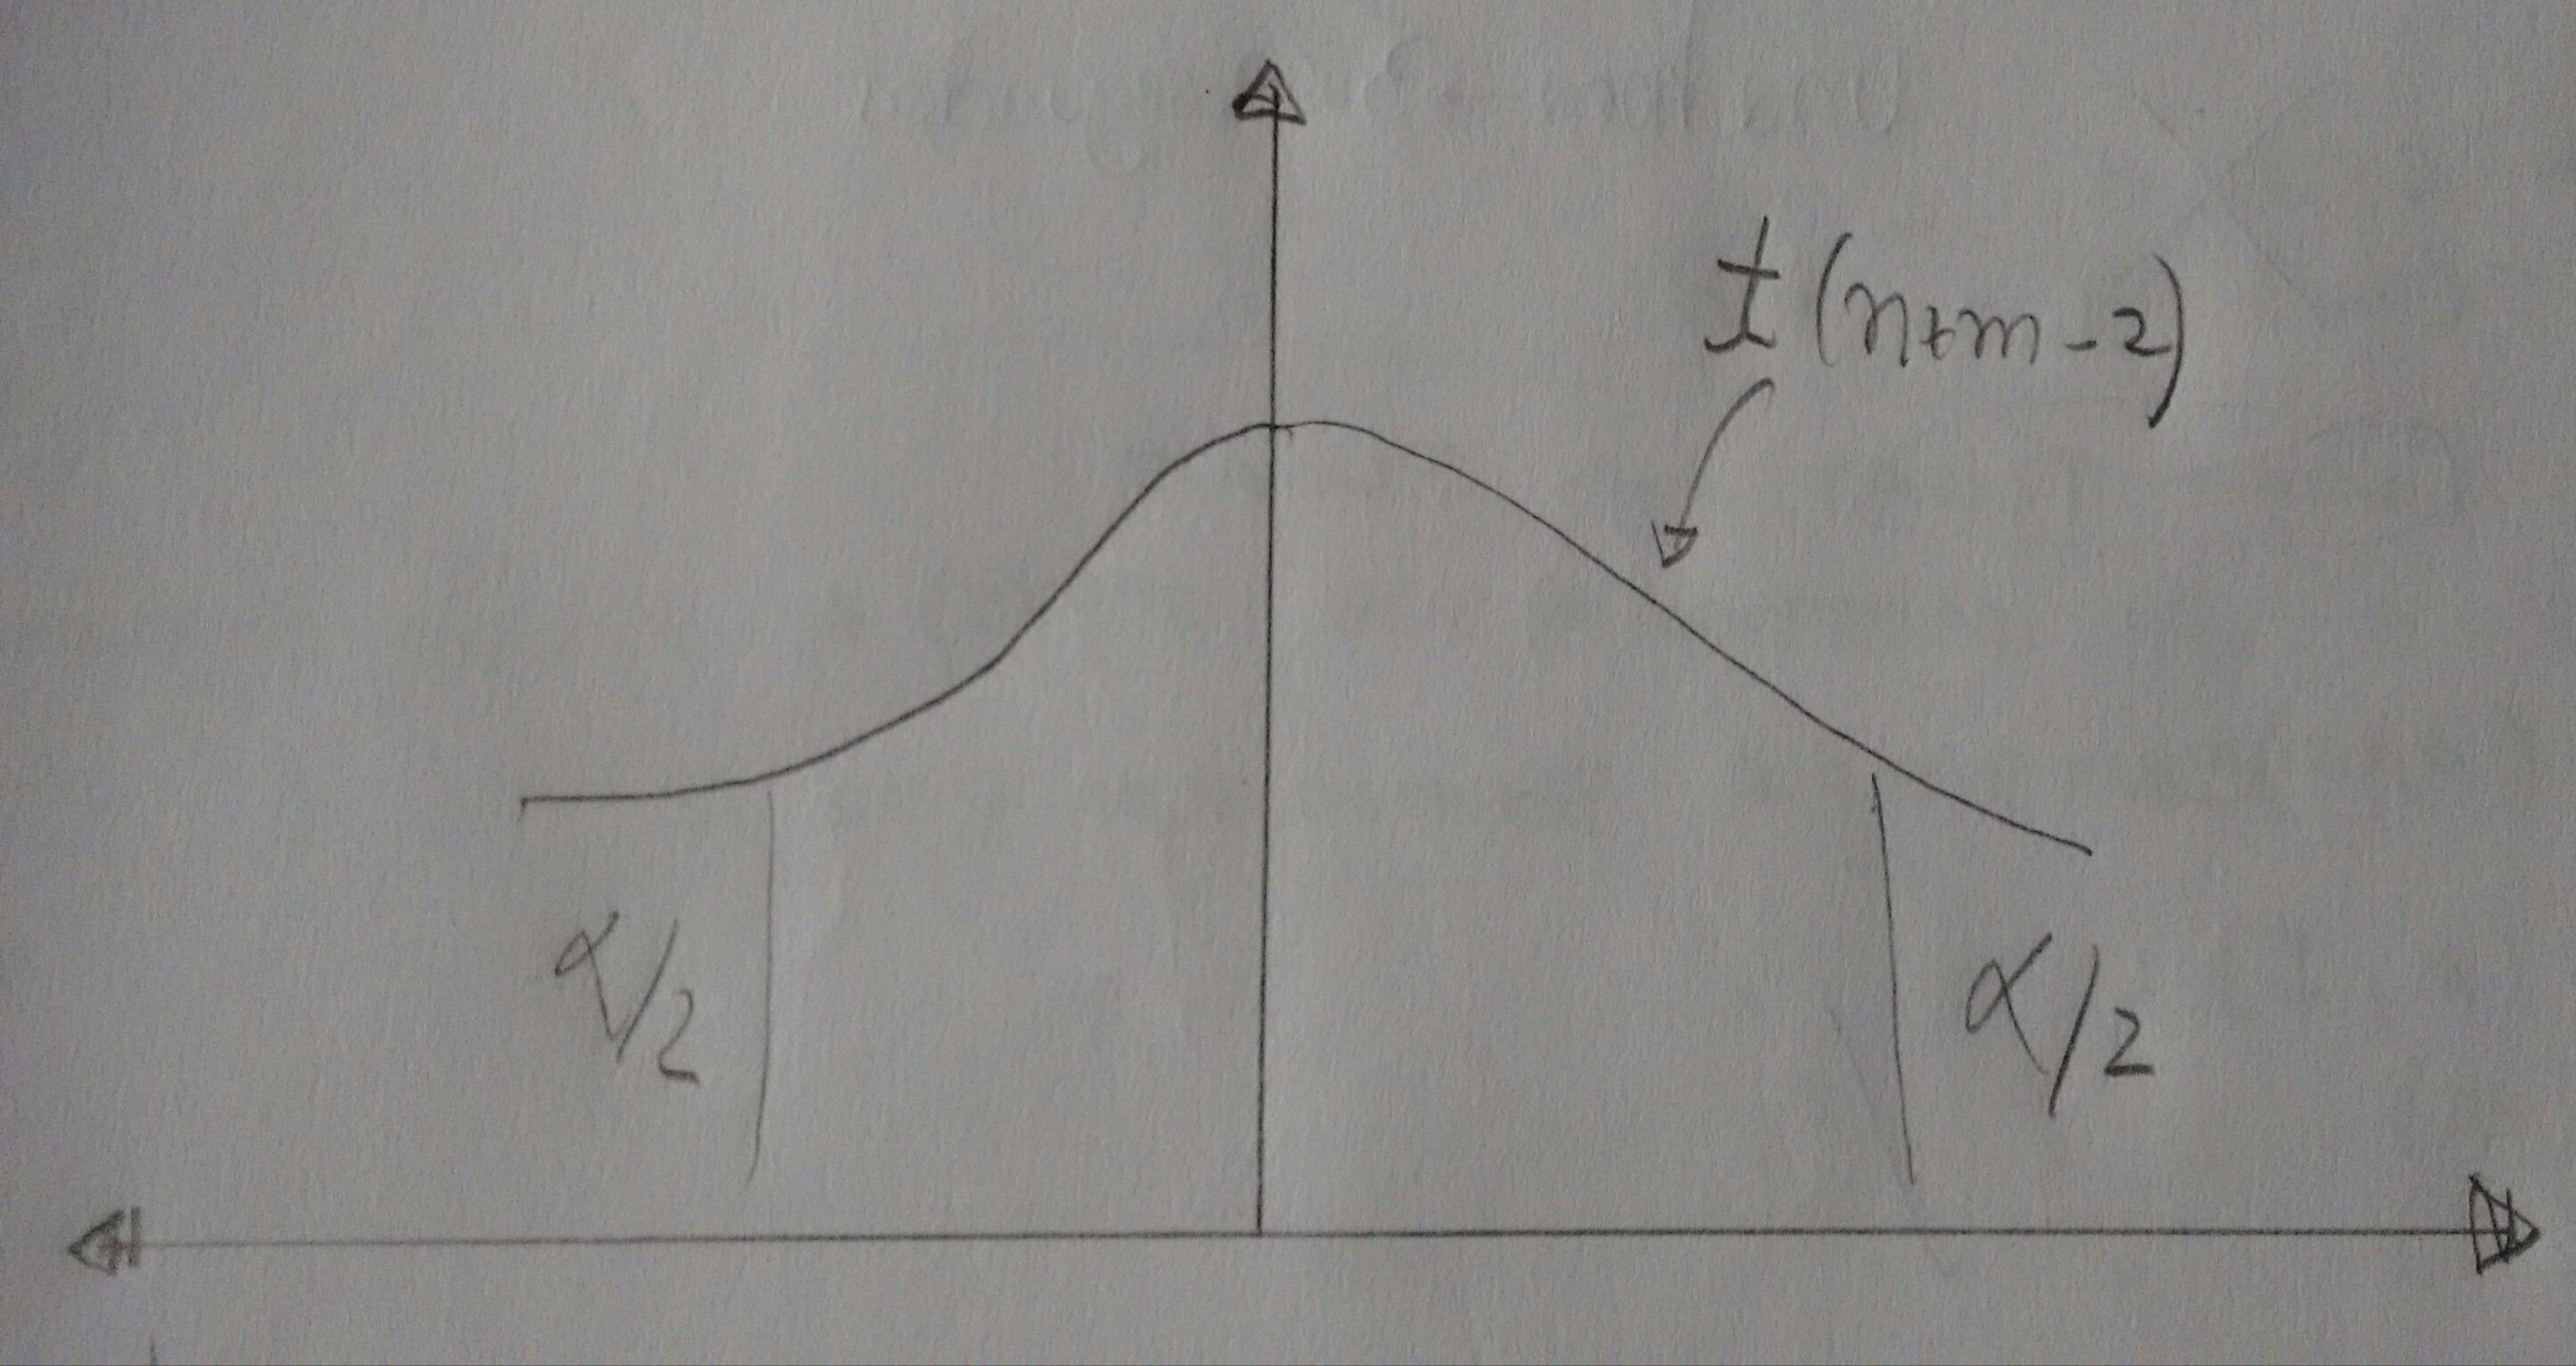
\includegraphics[scale=0.1]{imagenes/student.jpg}
\end{center}
\section{Complementos de test de hipótesis}
Hay un tema interesante que mencionamos, se trata de la propiedad de la razón de verosimilitud monótona. Gracias a esta propiedad se puede escribir de inmediato un test UMP pata un problema unilateral (sin aplicar TRV).\\

Una familia de densidades $f_{\theta}(X)$ y parámetro real $\theta$ tal que $\theta \not = \theta' \Rightarrow f_{\theta}(X) \not = f_{\theta'}(X)$ (idenficabilidad), se dice que posee razón de verosimilitud monótoma si $\forall \theta < \theta'$ el cociente $\frac{f_{\theta'}(X)}{f_{\theta}(X)}$ es función creciente de un estadístico $T(X)$

\begin{teo}
Si queremos testear  $H_{0}: \theta \le \theta_{0}$ versus $H_{1}:\theta>\theta_{0}$ y la familia $f_{\theta}(X)$ posee la propiedad de RVM entonces el test
\begin{align*}
\phi(X) =%
   \begin{cases}
    1  & T(X)>c \\
    \gamma & T(X) = c \\
    0 & T(X) < c
  \end{cases}
\end{align*}
donde $c,\gamma$ se calculan de forma que $\mathbb{E}_{\theta_{0}}(\phi(X)) = \alpha$ es UMP de nivel $\alpha$.
\end{teo}

Un ejemplo importante de RVM es la familia exponencial
\begin{align*}
f_{\theta} = c(\theta)e^{\underbrace{Q(\theta)}{\text{cociente en $\theta$}}T(X)}h(X)
\end{align*}
\begin{itemize}
\item $H_{0}: \theta = \theta_{0}$ versus $H_{1}: \theta \not= \theta_{0}$ no existe UMP
\item $H_{0}: \theta \in [\theta_{0},\theta_{1}]$  versus $H_{1}: \theta \not\in [\theta_{0},\theta_{1}]$ no existe UMP
\item $H_{1}: \theta \in [\theta_{0},\theta_{1}]$  versus $H_{0}: \theta \not\in [\theta_{0},\theta_{1}]$ si existe UMP
\end{itemize}
\end{document}